%\documentclass[iop]{emulateapj-rtx4}
% \shortauthors{French $\&$ Wakker}
%
%\usepackage{graphicx}
%\usepackage{subfigure}
%\usepackage{hyperref}
%\usepackage{amsmath}


%%%%%%%%%%
\documentclass[twocolumn,tighten]{aastex62}
%\documentclass{aastex6}
%\usepackage{emulateapj-rtx4}
%\usepackage{emulateapj}

 \shortauthors{French $\&$ Wakker}
\usepackage{graphicx}
\usepackage{subfigure}
\usepackage{amsmath}

%\usepackage{dblfloatfix}

%\usepackage{longtable}
%\usepackage{deluxetable}


\newcommand{\kms}{$\rm km\, s^{-1}$}
\newcommand{\HI}{\mbox{H\,{\sc i}} }

%\newcommand{\HI}{H\,{\sc i}}


\newcommand{\I}{\,{\sc i}}
\newcommand{\II}{\,{\sc ii}}
\newcommand{\III}{\,{\sc iii}}
\newcommand{\IV}{\,{\sc iv}}
\newcommand{\V}{\,{\sc v}}
\newcommand{\VI}{\,{\sc vi}}


\graphicspath{{figures//}}

\begin{document}

%\title{The environmental dependence of low-$z$ Ly$\alpha$ absorption}
\title{INTRODUCTION}


%Do Ly$\alpha$ absorbers co-rotate with galaxies?}

\author{David M. French}

\affil{Department of Astronomy, University of Wisconsin, Madison, WI 53706, USA}

\begin{abstract}

Galaxies must accrete gas from the intergalactic medium (IGM) in order to sustain star formation at observed levels. In order to understand this complex process, and how it influences galaxy evolution globally, it is necessary to understand the physical conditions and distribution of the gas around galaxies, known as the circumgalactic medium (CGM). This thesis aims to address these questions through the largest-to-date survey of low column density $\rm Ly\alpha$ absorption detected in the spectra of background QSOs taken by the Cosmic Origins Spectrograph (COS) on the Hubble Space Telescope (HST). By correlating the positions of detection absorption lines with the surrounding galaxy environment, I aim to gain insights to the complex relationship between intergalactic gas and the galaxies which feed on it. This introduction provides some historical and astrophysical perspective, as well as an overview of the methods and history of QSO absorption line spectroscopy.

\end{abstract}

\keywords{galaxies:intergalactic medium, galaxies:evolution, galaxies:halos, quasars: absorption lines}


\section{Overview of the Circumgalactic Medium}

The majority of the baryons in the universe are found in the diffuse intergalactic medium (IGM). The IGM and the galaxies that reside in it are tightly linked by processes such as feedback and accretion. In order to sustain the level of star formation observed, galaxies must accrete gas throughout their lifetimes (e.g., \citealt{erb2008, putman2009a, putman2009b, prochaska2009, bauermeister2010, genzel2010}). At the same time, ongoing star formation and active galactic nuclei (AGN) activity produce feedback that drives gas back into the IGM. This life cycle of gas is complex, and difficult to constrain observationally. Understanding the properties of the IGM, such as its densities, temperatures, motions, and its relationship to the galaxies embedded within it is \emph{essential} for explaining the evolution of galaxies and the star formation history of the Universe. 

The properties of the vast reservoir of material in the IGM can be understood by analyzing lines of sight toward background quasi-stellar objects (QSOs). Individual concentrations of gas along a given sightline imprint a `forest' of absorption lines on the spectrum in the direction of the QSO target. The metal lines trace the star formation history within the intervening gas, and neutral hydrogen lines ($\rm Ly\alpha$ is one of the most commonly and easily observed) indicate both the location and velocities of outflowing gas, as well as the presence of fuel for future star formation. Figure \ref{cgm_artist} shows an artists impression of a galaxy complete with a CGM halo with arrows indicating outflowing and recycling material, and an illustration of a HST sightline detecting halo gas absorption. The relationship between the galaxies and the IGM is usually studied by looking for galaxies that lie at similar redshifts as detected absorption lines. This approach has value but is incomplete; it does not allow for an unbiased understanding of the distribution of the gas around galaxies, which requires looking for both detections and non-detections of gas, both near as well as far away from galaxies.

The current standard model of structure formation is given by Lambda Cold-Dark-Matter ($\Lambda$CDM) cosmology, which predicts the hierarchical growth of large scale structures seeded by initial fluctuations in the dark matter background. In this picture, both galaxies and the IGM should follow the same underlying density profile. Some observational evidence of this large-scale relationship has appeared recently, such as \cite{wakker2015}, who showed that $\rm Ly\alpha$ absorption strength (equivalent width; EW) traces the overall distribution of galaxies in a Cosmic Web filament. Figure \ref{wakker_filament} shows their plot of the EW of $\rm Ly\alpha$ absorbers as a function of distance to the center of a galaxy filament, with the enhanced absorption strength evident close to the filament center. In addition, numerous studies have shown that $\rm Ly\alpha$ absorbers also trace individual galaxy halos (e.g., \citealt{lanzetta1995, chen1998, chen2001a,  tripp1998, bowen2002, cote2005, wakker2009, steidel2010, prochaska2011, thom2012, stocke2013, liang2014, danforth2016})


\begin{figure}[ht!]
        \centering
        \vspace{0pt}
        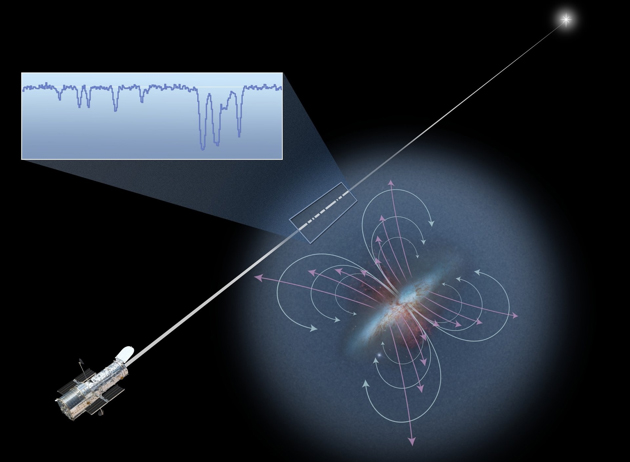
\includegraphics[width=0.49\textwidth]{hubble_cgm.jpg}
        \caption{\small{An artist's impression of the CGM of a galaxy. Image credit: NASA/STScI/Ann Feild}}
        \vspace{5pt}
        \label{cgm_artist}
\end{figure}


\begin{figure}[ht!]
        \centering
        \vspace{0pt}
        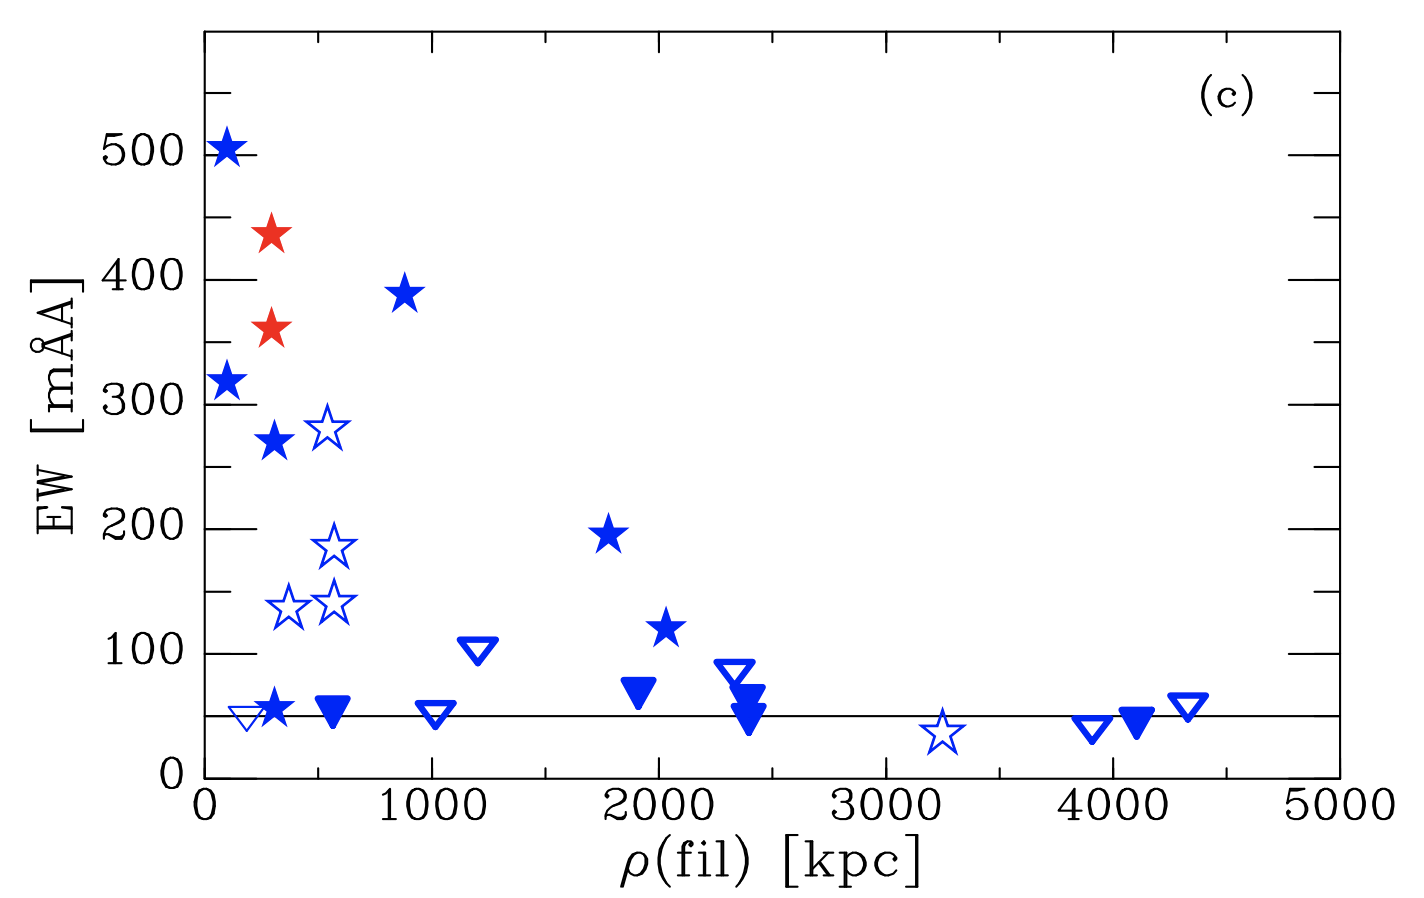
\includegraphics[width=0.49\textwidth]{Wakker2015_filament_EW.png}
        \caption{\small{The EW of $\rm Ly\alpha$ absorbers as a function of distance to the center of a galaxy filament. Blue downward tracing triangles indicate upper limits for non-detection, and all stars indicate detections. See \cite{wakker2015}.}}
        \vspace{5pt}
        \label{wakker_filament}
\end{figure}

The majority of these studies have reported tentative evidence for enhanced $\rm Ly\alpha$ absorption strength with increasing galaxy proximity. \textbf{NEED TO MENTION COS-Halos}.


Recent studies find that about half of $\rm Ly\alpha$ absorbers lie within galaxy halos, at impact parameters $\rho \lesssim 350$ kpc \citep{cote2005, prochaska2006}. In addition, \cite{wakker2009} find that for 90\% of $L > 0.1 L^{\**}$ galaxies an absorber can be found within 400 kpc and 400 \kms~, and all galaxies have a $\rm Ly\alpha$ absorber within 1.5 Mpc. Higher redshift studies, such as \cite{rudie2012a} at $2 < z < 3$, find evidence for an elevated density of absorbers up to 2 Mpc from galaxies. \cite{wakker2009} also confirmed a previously suggested correlation between $\rm Ly\alpha$ absorption linewidth (also called Doppler $b$-parameter) and impact parameter ($\rho$), observing that the broadest lines (FWHM $>150$ \kms) are only seen within 350 kpc of a galaxy, while only narrower lines (FWHM $<75$ \kms) are found at $\rho > 1$ Mpc (see Figure \ref{wakker2009_linewidth}).


\begin{figure}[ht!]
        \centering
        \vspace{0pt}
        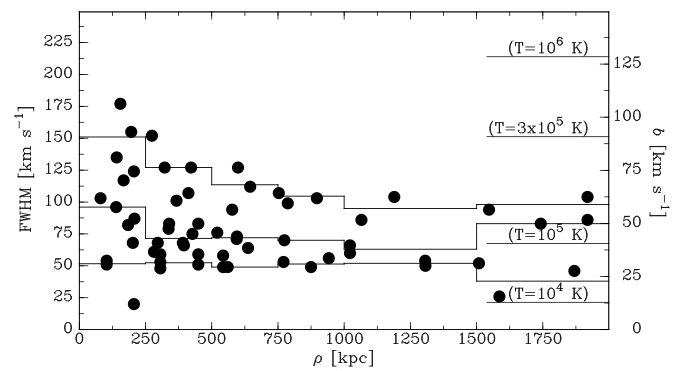
\includegraphics[width=0.49\textwidth]{bart_moneyplot.png}
        \caption{\small{The linewidth (or Doppler $b$-parameter) and FWHM of $\rm Ly\alpha$ absorbers as a function of physical impact parameter to the nearest galaxy. Histograms show the 10th, 50th, and 90th percentiles of the distribution.  See \cite{wakker2009}.}}
        \vspace{5pt}
        \label{wakker2009_linewidth}
\end{figure}

In addition, studying the enrichment of galaxy halos is necessary for constraining outflow models and informing stellar feedback prescriptions. Directly measuring the velocity field and column densities of absorbers as a function of impact parameter and orientation around galaxies would provide the clearest evidence of inflow or outflow activity, but results are few and uncertain. \cite{kacprzak2011_inclination} claim to find that Mg\II~ equivalent widths correlate with galaxy inclination but \cite{mathes2014} find no such correlation for $\rm Ly\alpha$ and O\VI absorbers. Furthermore, we should expect outflowing gas to be more highly enriched and trace the metallicity of the associated galaxy, with inflowing gas instead appearing only in \HI. Both \cite{stocke2013} and \cite{liang2014} find an ``edge" to heavy ion absorption at $\sim 0.5 R_{\rm vir}$, but with $\rm Ly\alpha$ covering fractions of $\sim 0.75 - 1$ continuing out to $R_{\rm vir}$. However, \cite{mathes2014} measure O\VI absorption out to $\sim 3 R_{\rm vir}$.

All these previous studies have suffered from small sample sizes (most with fewer than 50 systems), and incompleteness due to their higher mean redshifts where it is increasingly difficult to detect faint galaxies surrounding absorption systems. This thesis aims to address some of these issues by compiling the largest-yet survey of $\rm Ly\alpha$ absorbers spread across a range of environments, and both near and far from galaxies. This project is focused on the nearby Universe ($cz \leq 10,000$ \kms), where the existing galaxy data is good and relatively complete to $\sim 0.1 L^{\**}$. In Chapter 1 I describe the compilation of a new nearby galaxy catalog to take advantage of this existing data. This catalog is then correlated with the over 700 archival QSO targets observed by the Cosmic Origins Spectrograph (COS) on the Hubble Space Telescope (HST) to produce a sample of galaxy-target systems including a range of galaxy environments, orientations, and types. In the following section I summarize the 3 major questions this thesis aims to tackle.

%The CGM is commonly split into a two gas phases: a hot, mostly collisionally ionized phase with gas temperatures near $T\gtrsim 10^6$ K, and a cool, mostly photoionzied phase with gas temperatures near $T \lesssim 10^4$ K.

%\cite{lanzetta1995, bowen1996, chen2008, steidel2010, prochaska2011b, wakker2009}



\section{Science Goals}
While there are numerous open questions concerning the interactions of galaxies and the gas that surrounds them, this thesis focuses on the following:

%1. \emph{Do the physical properties of absorbers depend on their location and orientation with respect to galaxies?}
%2.
%3.
%4.

\subsection{Galaxy Proximity}
\emph{How strongly is intergalactic gas concentrated near galaxies, and does the presence of galaxies appear affect the physical properties of absorbers?} Recent studies find that half of all $\rm Ly\alpha$ absorbers lie within galaxy halos, at impact parameters of $\rho <350$ kpc and within $400$ \kms~of a galaxy (e.g., \citealt{cote2005, prochaska2006, wakker2009}). Furthermore, \cite{sorini2018} find that the ``sphere of influence" of galaxy can extend all the way to $\sim 2$ Mpc, far more distant than the $\sim150$ kpc or $\sim 1 R_{\rm vir}$ often used as the search radius for CGM studies. The properties of the lines also appear to change with impact parameter. For example, it has been known for some time that higher column density absorption is found closer to galaxies, and there is good evidence that the same is true for absorption linewidth and FWHM (e.g., \citealt{wakker2009, prochaska2011}). However, it remains unclear which physical process is responsible; increased turbulence, temperature, ionizing radiation field, or an effect of velocity gradients or blending of multiple cloudlets along the line of sight. Studying this phenomenon as a function of environment with good understanding of the properties, morphologies, and group memberships of the nearby galaxies is the clearest way forward on this question, and a larger statistical sample then previously employed will be required.


\subsection{Galaxy Orientation}
\emph{Do the physical properties of absorbers depend on their orientation with respect to nearby galaxies?} Recent results suggest that absorbing systems have a preferred orientation with respect to the major and minor axes of the galaxies they are near to (e.g., \citealt{kacprzak2011_inclination, kacprzak2012}. This could be evidence of inflows and outflows, an effect of the global structure of galaxy halos, or a signature of a preferred orientation of galaxy halos within Cosmic Web filaments. Unfortunately the statistics are not yet good enough to distinguish between these possible scenarios. Additionally, very few authors (see, e.g., \cite{mathes2014, bordoloi2014}) have investigated the dependence of absorber properties on nearby galaxy \emph{inclination}, the results of which could have important implications for galaxy halo shape and the spatial dependence of halo gas covering fractions. A large-scale study into the inclination and azimuth angle dependence of absorption is the clearest path forward here.

%\cite{mathes2014} and \cite {bordoloi2011} find little evidence for inclination dependence for O\VI and Mg\II absorbers, but the models of \cite{bordoloi2014} predict 

\subsection{Galaxy Rotation}
\emph{Does intergalactic gas ``know" about the rotation of the galaxies embedded within it?} In particular we would like to know how far out (or to what impact parameter) the rotational curves of galaxies extend, or in other words what angular momentum information is retained by galaxy halos. Previous studies (e.g., \citealt{steidel2002, cote2005, wakker2009, kacprzak2011_kinematics}) were unable to find a clear correlation between the rotation of galaxy disks and the kinematics of nearby absorbers. However, none of these previous studies have been able to produce a sample of more than a handful of systems, and have only considered the possibility of an extended, warped stellar disk in their analysis. A targeted observational campaign for easily observed galaxies in the local Universe could make substantial progress here.


\section{Summary of Thesis}
In the following chapters I describe a program to observationally explore the connections between low column density $\rm Ly\alpha$ absorption and the galaxy environment in the local Universe. This program focuses mainly on archival QSO observations taken by the Cosmic Origins Spectrograph (COS) on the Hubble Space Telescope (HST), and correlations between the locations of detected $\rm Ly\alpha$ absorption and of galaxies larger than $\sim 0.1 L^{\**}$. By restricting our study to low-redshifts ($cz \leq 10,000$ \kms) we are able to compile a dataset of unparalleled size while remaining highly complete to galaxies of all types, sizes, and distances from absorption detections. The results of this thesis are presented as follows:

1. In Chapter 1 I present a new nearby galaxy catalog. In order to study the CGM-galaxy connection on a large, all-sky scale, we rely heavily on archival, publicly available data for the positions and properties of the galaxies. We describe the retrieval, handling, homogenization and completeness of these data, as well as detailed descriptions of each included galaxy property (i.e., the catalog columns).

 
2. In Chapter 2 I present the results of a pilot study with 33 QSO sightlines chosen for their proximity to large galaxies ($D \ge 25$ kpc). We introduce a new method for absorber-galaxy matching called the likelihood-method, which will make it possible to algorithmically study our large final data set. Using this likelihood-method we match 48 $\rm Ly\alpha$ absorption lines with nearby large galaxies, and study the absorption strength (EW) as a function of velocity and spatial separation, azimuth angle and inclination. We find that the strongest absorbers are all found within $100$ \kms~of a galaxy, and that there exists an overabundance of detections near highly inclined galaxies ($inc \gtrsim 50^{\circ}$). We attribute this overabundance to the effect of flattened, non-spherical galaxy halos on the detection probability as a function of impact parameter.


3. In Chapter 3 I present the results of a study of the kinematic connection between galaxy disks and $\rm Ly\alpha$-traced halo gas. We have compiled a sample of 29 galaxies with known rotation curves both from the literature and from new observations with the Southern African Large Telescope (SALT) which also appear within $3 R_{\rm vir}$ of a COS QSO sightline. We compare the galaxy disk kinematics to the velocities of $\rm Ly\alpha$ absorption lines detected in 19 nearby QSO sightlines with the help of custom cylindrical and NFW-based halo rotation models \citep{navarro1996, navarro1997}. We find that the co-rotation fraction of absorbers declines as a function of galaxy luminosity, which we attribute to the effect of cold-mode accretion dominating in lower-mass galaxy halos.


4. In Chapter 4 I present the results of our full CGM survey, which includes 1135 $\rm Ly\alpha$ absorbers detected in the spectra of 264 QSO spectra. We explore the effect of different normalizations to our likelihood-method for absorber-galaxy matching, and use this technique to split absorber-galaxy systems into 5 different bins based on their galaxy environments. We find that both absorption strength (EW) and linewidth (Doppler $b$-parameter) are enhanced with proximity to a single galaxy, and further enhanced by proximity to multiple galaxies. We also detect a bimodal azimuth distribution, with $\rm Ly\alpha$ absorbers preferentially found slightly offset from both the minor and major galaxy axes. We confirm the inclination results first suggested in Chapter 2.

5. In Chapter 5 I summarize the results of this thesis, and place these results in the broader context of the circumgalactic medium and it's implications for global galaxy evolution.



%\nocite{*}
%\bibliography{rotation_bib}
%\bibliography{/Users/frenchd/Research/bib}{}
\bibliography{/Users/frenchd/Research/inclination/git_inclination/bib}{}
\bibliographystyle{apj}

\clearpage

\end{document}
